\documentclass[a4paper, 12pt]{report}

\title{Éditeur web}
\author{Pierre Burc, Olivier Duplouy, Hamza Erraji, Issame Amal, Mickaël Berger, Joachim Divet, Zaydane Sadiki & Abdelhamid Belarbi}

%% Pour des marges plus équitables.
\usepackage[margin=1.5cm]{geometry}
%% Pour la langue des titres et sous-titres.
\usepackage[francais]{babel}
%% Pour de belles images.
\usepackage{graphicx}
%% Pour la police de caractères.
\usepackage{fontspec}
\setmainfont{Delicious-Roman}
%% Pour faire le glossaire.
\usepackage[xindy]{glossaries}
\makeglossaries
%% Pour les notes de bas de page.
\usepackage{fmtcount}
%% Pour pouvoir écrire du code.
\usepackage{minted}
\usemintedstyle{tango}
\definecolor{bg}{rgb}{0.95,0.95,0.95} %% Pour le background du code.
\renewcommand{\theFancyVerbLine}{\sffamily \textcolor[rgb]{0.5,0.5,1.0}{\scriptsize \oldstylenums{\arabic{FancyVerbLine}}}}
\newminted{cpp}{linenos=true,bgcolor=bg,frame=lines}
\begin{document}
	%% Glossaire
	\newglossaryentry{UML}
	{
		name={UML},
		description={Unified Modeling Language, langage de modélisation graphique à base de pictogrammes}
	}

	\newglossaryentry{diagramme de Gantt}
	{
		name={diagramme de Gantt},
		description={Le diagramme de Gantt est un outil utilisé en ordonnancement et gestion de projet et permettant de visualiser dans le temps
		les diverses tâches liées composant un projet. Il permet de représenter graphiquement l'avancement du projet}
	}
	
	\newglossaryentry{bogue}
	{
		name={bogue},
		description={En informatique, un bug (de l’anglais bug, « insecte ») ou bogue est un défaut de conception d'un programme
		informatique à l'origine d'un dysfonctionnement},
		plural={bogues}
	}
		
	\newglossaryentry{Qt}
	{
		name={Qt},
		description={C'est un framework orienté objet et développé en C++. Il offre des composants d'interface graphique (widgets),
		d'accès aux données, de connexions réseaux, de gestion des fils d'exécution, d'analyse XML, etc}
	}

	\newglossaryentry{gestionnaire de version}
	{
		name={gestionnaire de version},
		description={La gestion de versions consiste à maintenir l'ensemble des versions d'un ou plusieurs fichiers (généralement en texte).
		Essentiellement utilisée dans le domaine de la création de logiciels, elle concerne surtout la gestion des codes source}
	}

	\newglossaryentry{Git}
	{
		name={Git},
		description={Un logiciel de gestion de versions décentralisé. 
		C'est un logiciel libre créé par Linus Torvalds, le créateur du noyau Linux, et distribué selon les termes de la licence 
		publique générale GNU version 2}
	}

	\newglossaryentry{WYSIWYG}
	{
		name={WYSIWYG},
		description={Un WYSIWYG est une interface utilisateur qui permet de composer visuellement le résultat voulu, typiquement 
		pour un logiciel de mise en page, un traitement de texte ou d’image. 
		C'est une interface « intuitive » : l’utilisateur voit directement à l’écran à quoi ressemblera le résultat final}
	}
	
	\newglossaryentry{autocomplétion}
	{
		name={autocomplétion},
		description={l'autocomplétion, est une fonctionnalité informatique permettant à l'utilisateur de limiter la quantité d'informations 
		qu'il saisit avec son clavier, en se voyant proposer un complément qui pourrait convenir à la chaîne de caractères qu'il a commencé à taper}
	}

	\newglossaryentry{expression régulière}
	{
		name={expression régulière},
		description={Une expression rationnelle ou expression régulière est en informatique une chaîne de caractères que l’on appelle parfois un motif
		et qui décrit un ensemble de chaînes de caractères possibles selon une syntaxe précise.
		Les expressions rationnelles sont issues des théories mathématiques des langages formels},
		plural={expressions régulières}
	}

	\newglossaryentry{MVC}
	{
		name={MVC},
		description={Le modèle-vue-contrôleur (en abrégé MVC, de l'anglais Model-View-Controller) est un patron d'architecture et une méthode de conception qui organise l'interface homme-machine (IHM) d'une application logicielle (voir chap. 7)},
		plural={expressions régulières}
	}

	\newglossaryentry{Html}
	{
		name={Html},
		description={L’Hypertext Markup Language, généralement abrégé Html, est le format de données conçu pour représenter les pages Web. C’est un langage de balisage qui permet d’écrire de l’hypertexte, d’où son nom}
	}

	\newglossaryentry{Php}
	{
		name={Php},
		description={Le Php : Hypertext Preprocessor, plus connu sous son sigle Php, est un langage de scripts libre principalement utilisé pour
		produire des pages Web dynamiques}
	}

	\newglossaryentry{JavaScript}
	{
		name={JavaScript},
		description={JavaScript est un langage de programmation de scripts principalement utilisé dans les pages web interactives}
	}

	\newglossaryentry{Css}
	{
		name={Css},
		description={(Cascading Style Sheets: feuilles de style en cascade) est un langage informatique qui sert à décrire la présentation
		des documents Html et XML}
	}

	\newglossaryentry{Doxygen}
	{
		name={Doxygen},
		description={Doxygen est un logiciel informatique libre permettant de créer de la documentation à partir du code source d'un programme.
		Pour cela, il tient compte de la grammaire du langage dans lequel est écrit le code source, ainsi que des commentaires s'ils sont écrits
		dans un format particulier}
	}

	\newglossaryentry{parseur}
	{
		name={parseur},
		description={L'analyse syntaxique consiste à mettre en évidence la structure d'un texte, généralement un programme informatique ou du texte
		écrit dans une langue naturelle. Un analyseur syntaxique (parser, en anglais) est un programme informatique qui réalise cette tâche}
	}

	\newglossaryentry{MDI}
	{
		name={MDI},
		description={En Informatique, Multiple Document Interface ou MDI désigne l'organisation de l'interface graphique d'une application où des
		fenêtres « parentes » contiennent en leur sein des fenêtres enfants. Le cas typique d'application consiste en la fenêtre principale de l'application, avec un menu et des barres d'outils, contenant une (sous-)fenêtre par fichier ou projet ouvert}
	}

	\newglossaryentry{Flex}
	{
		name={Flex},
		description={Flex est un outil pour générer des analyseurs, programmes qui reconnaissent des motifs lexicaux dans du texte}
	}

	\newglossaryentry{Bison}
	{
		name={Bison},
		description={GNU Bison est l'implémentation de l'analyseur syntaxique yacc par le projet GNU}
	}

	\newglossaryentry{Valgrind}
	{
		name={Valgrind},
		description={Valgrind (prononcé [vælɡrɪnd], et non [vælɡraɪnd]1) est un outil de programmation libre pour déboguer, effectuer du profilage 
		de code et mettre en évidence des fuites mémoires}
	}

	\newglossaryentry{C++}
	{
		name={C++},
		description={Le C++ est un langage de programmation permettant la programmation sous de multiples paradigmes comme la programmation
		procédurale, la programmation orientée objet et la programmation générique. C++ est actuellement le 4e langage le plus utilisé au monde}
	}

	\begin{titlepage}
		\center{
\includegraphics[width=5cm]{images/logoUM2.png}}\\ 
		~\\
		~\\
		~\\
		~\\
		~\\		
		\begin{center}
			{\large Rapport de projet} \\
			{\large Licence 3}\\
			\vspace{1,5cm}
			{\Huge Editeur de sites web}\\
			~\\
			~\\
			~\\
			
\includegraphics[width=12.5cm]{images/logoTest1.png}
			~\\
			~\\
			{\large Réalisé par :} \\
			~\\
			{\LARGE Pierre Burc, Olivier Duplouy, \\
				      Hamza Erraji, Issame Amal,\\
				      Mickaël Berger, Joachim Divet,\\
				      Zaydane Sadiki et Abdelhamid Belarbi}\\
			\vspace{1,5cm}
			{\large Sous la direction de :} \\
			~\\
			{\LARGE Michel Meynard} \\
			\vspace{2.5cm}
			{\large Année universitaire 2011-2012 }			
		\end{center}
	\end{titlepage}
%%%%%%%%%%%%%%%%%%%%%%%%%%%%%%%%%%%%%%%%
%%%%%%%%%%%%%%%%%%%%%%%%%%%%%%%%%%%%%%%%
	\begin{chapter}*{Remerciements}
	Nous tenons à remercier tout particulièrement M. Michel Meynard, notre tuteur de projet qui nous a guidés et épaulés tout au long de
	ces quelques mois de travail, égrénant ça et là différents conseils utiles à souhait. \\

	Bien entendu nous n'oublions pas de remercier chaleureusement toute l'équipe pédagogique de l'UM2 qui nous a apporté son soutien.\\

	Et il va sans dire que tous les membres du groupe se remercient les uns les autres.
	\end{chapter} 
%%%%%%%%%%%%%%%%%%%%%%%%%%%%%%%%%%%%%%%%
%%%%%%%%%%%%%%%%%%%%%%%%%%%%%%%%%%%%%%%%
	%% Table des matières.
	\tableofcontents
	%% Table des figures
	\listoffigures
	%% Table des tables
	\listoftables
%%%%%%%%%%%%%%%%%%%%%%%%%%%%%%%%%%%%%%%%
%%%%%%%%%%%%%%%%%%%%%%%%%%%%%%%%%%%%%%%%
	\begin{chapter}*{Introduction}
	\addcontentsline{toc}{chapter}{Introduction}

	C'est par une froide journée d'hiver que nous nous réunîmes pour la première fois à l'université de Montpellier. 
	Huit, tous étudiants préposés au projet numéro vingt-trois nous attendons à notre table l'arrivée de notre tuteur M. Meynard. 
	Ce dernier se présente, nous salue et prononce ce discours mémorable qui restera gravé dans nos mémoires.\\
	\begin{quotation}
		« Dans le cadre de développement de sites Web, on souhaiterait utiliser un éditeur multi-fichiers permettant de réaliser 
		différentes actions sur	des fichiers relatifs à un site : édition de fichiers \gls{Html}, \gls{Php}, \gls{JavaScript} et \gls{Css}.\\

		Il serait également appréciable que cet éditeur proposât un mode de visualisation du site dans un navigateur et un mode arborescence.\\

		Et tant que nous y sommes, mettons de l'\gls{autocomplétion}, de la coloration syntaxique, un accès aux manuels
		des langages cités précédemment et une validation \gls{Html}. ».
	\end{quotation}

	Après ce laïus prononcé d'une traite M. Meynard disparut soudain, nous laissant là, le regard vide.\\


	Néanmoins, nous nous remîmes assez vite de notre ahurissement et un sage parmi nous s'écria soudain :
	\begin{quotation}
		« Nous commencerons par étudier quelques éditeurs existants sur le marché pour nous faire une idée. Ensuite nous concevrons
		le programme avec le langage UML en nous organisant pour la réalisation.
		Enfin, nous implémenterons l'application insolents et sûrs de nous.	Qu'en dites-vous ? ».
	\end{quotation}

	Nous n'en dîmes que du bien. En effet, l'idée loin d'être incroyablement novatrice avait l'avantage d'être logique et cohérente.\\


	C'est ainsi que démarra le projet \emph{Éditeur web} décrit dans ce document, entrons donc sans plus attendre dans le vif du sujet.
	
	\end{chapter}
%%%%%%%%%%%%%%%%%%%%%%%%%%%%%%%%%%%%%%%%
%%%%%%%%%%%%%%%%%%%%%%%%%%%%%%%%%%%%%%%%
	\begin{part}{Analyse}
		\begin{chapter}{Cahier des charges}
			Voici une liste exhaustive des fonctionnalités prescrites par M. Meynard :
			\begin{itemize}
				\item Édition des fichiers \gls{JavaScript}, \gls{Php}, \gls{Css} et \gls{Html} ;
				\item Un système multi-onglets permettant de naviguer rapidement entre plusieurs fichiers d'un même projet ;
				\item Possibilité de visualiser le site sous forme d'arborescence ;
				\item Mode \gls{autocomplétion} et coloration syntaxique ;
				\item Mode auto-indentation ;
				\item Accès en un clic au manuel \gls{Php}/\gls{Html}/\gls{Css}/\gls{JavaScript} ;
				\item Validation \gls{Html} ;
				\item Visualisation du site dans un navigateur ;
				\item Squelette de site préexistant.
			\end{itemize}~\\

			La liste d'exigences ci dessus se résume en une besoins graphiques, il nous fallait donc « deviner » ce qui se déroule en interne 
			dans le programme. Malgré les différents avis données par M. Meynard, il était difficile pour la majorité des membres de
			comprendre comment fonctionnait un tel programme.\\

			Après plusieurs colloques, discussions, palabres et réunions, il fut décidé que le meilleur moyen de se rendre compte de ce que
			représentait un tel cahier des charges en terme de produit fini était d'étudier les différents éditeurs existants offrants ce 
			genre de fonctionnalités.
		\end{chapter}

		\begin{chapter}{Étude de projets existants}
		\begin{section}{Espresso}
				\begin{figure}[h]
					\begin{center}
						
\includegraphics[width=3cm]{images/logoEspresso.png}
						\caption{Espresso}
					\end{center}
				\end{figure}~\\
				Le premier programme d'édition de site web que nous avons étudié propose les mêmes fonctionnalités que le
				logiciel que nous nous proposons de développer, à savoir coloration syntaxique, indentation automatique, arborescence des codes, etc.
				Il sera à priori une bonne source d'inspiration pour nous d'autant plus que l'interface est très soignée et agréable d'utilisation.
			\end{section}
			~\\
			\begin{section}{Aptana}
				\begin{figure}[h]
					\begin{center}
						
\includegraphics[width=4cm]{images/logoAptana.png}
						\caption{Aptana}
					\end{center}
				\end{figure}~\\
				Cet éditeur propose un ensemble de fonctionnalités nombreuses et variées. 
				Beaucoup plus fourni que Espresso, il propose des fonctionnalités complexes dans divers langages : 
				déboguage, déploiement automatique, gestionnaire de version inclus, terminal intégré et moult autres outils.
				Pour nous c'est un bon modèle à suivre en évitant tout de même de tomber dans le piège du sur-nombre d'options 
				qui importuneraient l'utilisateur. 
			\end{section}
			~\\
			\begin{section}{Dreamweaver}
				\begin{figure}[h]
					\begin{center}
						
\includegraphics[width=3cm]{images/logoDreamweaver.png}
						\caption{Dreamweaver}
					\end{center}
				\end{figure}~\\
				Dreamweaver est une référence en la matière. Il réunit les atouts des deux éditeurs sus-cités en joignant l'utile à l'agréable.
				Il possède en outre un mode dit \gls{WYSIWYG} permettant de dessiner l'interface d'un site web.
			\end{section}
			~\\


			\begin{section}{Bilan comparatif}
				Le tableau \ref{comparatif}, donne la distributions de quelques fonctionnalités parmi les logiciels cités précédemment. Il est
				inutile de mettre dans ce tableau des fonctionnalités telles que la coloration ou l'édition de fichier, car il est évident que des
				lesdits logiciels possèdent ce genre de spécificités.\\

				%% Ajout d'une petite note de bas de page.
				\addtocounter{footnote}{1}
				\footnotetext[\value{footnote}]{À noter que l'auto-indentation dans le tableau \ref{comparatif} concerne la capacité de 
				formater tout un fichier et non pas d'ajouter une tabulation après saut de ligne.}
				\begin{table}[h]
				\caption{\label{comparatif} Fonctionnalités spéciales dans les éditeurs étudiés}
					\begin{tabular}{|c||c|c|c|c|c|} % c signifie center, le texte de chaque colonne sera donc centré.
					  \hline
					  Éditeur & onglets & autocomplétion & auto-indentation$^{\decimal{footnote}}$ & validation \gls{Html} & documentations \\
					  \hline

					  Espresso & oui & oui & non & non & non \\
					  Aptana & oui & oui & non & oui & oui \\
					  Dreamweaver & oui & oui & oui & oui & non \\
					  \hline
					\end{tabular}
				\end{table}

				Ainsi, il ressort du tableau \ref{comparatif} qu'aucun des outils étudiés ne possède toutes les spécificités de notre programme.
				Il faudra donc, si nous voulons de l'inspiration, naviguer d'un éditeur à l'autre selon que nous voulons implémenter telle ou
				telle fonctionnalité.\\


				Maintenant que l'objectif est discernable et que le groupe a une idée générale du logiciel à produire, il est temps de
				penser à choisir les outils à utiliser.
			\end{section}
		\end{chapter}
		\begin{chapter}{Choix des outils}
			Il est des choix qui influent sur l'ensemble d'un projet et le choix des outils est de ceux là.
			Nous nous devions de faire un choix judicieux compte tenu de différents critères, à savoir la taille de l'équipe (huit personnes),
			l'ampleur du projet, le temps imparti et autres menus détails.\\


			La modélisation formelle des spécifications du programme nécessite un langage adapté à ce genre de besoin. C'est donc presque
			sans discussion que nous prîmes l'évidente décision d'utiliser le langage UML pour ce faire.
			Les diagrammes seront dessinés grâce à une application web nommée yUML (cf. sitographie, p.\pageref{sitographie}).\\


			Concernant le langage de programmation principal, nous choisîmes \gls{C++}.
			Ce choix est motivé par deux raisons, d'une part nous apprenons actuellement ce langage en cours, d'autre part,
			il s'agit d'un langage stable, documenté et qu'il fait bon d'avoir dans sa besace.\\


			Après cela M. Meynard nous proposa le framework \gls{Qt}. Un peu austère de prime abord, presque effrayant, il s'avéra finalement très
			sympathique grâce notamment à une syntaxe lisible et à une documentation bien feuillue.\\

			Pour générer une documentation de notre code source, nous fîmes le choix de \gls{Doxygen}, un outils spécialisé dans ce genre
			de tâches.\\


			Pour travailler en équipe sur un projet de ce genre il est utile voire indispensable de disposer d'un outil de synchronisation et
			de partage. Notre choix s'est porté sur le gestionnaire de version \gls{Git}. Ceci sans raison particulière car ses semblables offrent
			des fonctionnalités similaires.\\


			Bien que les huit membres de notre groupe furent géographiquement proches à vol d'oiseau, aucun d'entre nous ne possédait l'étonnante
			capacité de se déplacer dans les airs. Par conséquent, hormis les outils sus-cités il fallut quelques outils auxiliaires de communication.
			\\
			Nous utilisâmes donc des outils web tels que :
			\begin{description}
				\item[MicroMobs.com :] Pour les discussions professionnelles ;
				\item[Facebook.com :] Pour les annonces importantes, les messages, les dates de réunions, etc.
			\end{description}~\\

			Citons aussi TeamGantt.com, une application qui permet de dessiner un (très joli) \gls{diagramme de Gantt} en ligne.
		\end{chapter}
		\begin{chapter}{Organisation}
			\begin{section}{Diagramme de Gantt}
				Le projet se déroulant sur quatre mois, il a fallu faire un planning qui s'étale sur ledit laps de temps.
				Voici toutes les étapes du projet inscrites sur un \gls{diagramme de Gantt}.
				\begin{figure}[h]
					\begin{center}
						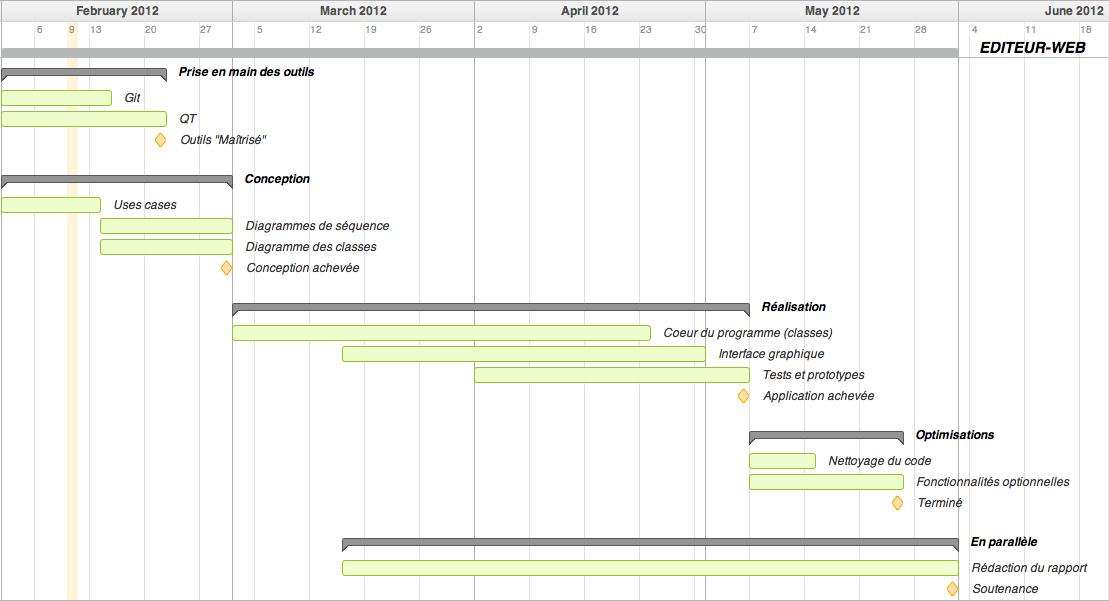
\includegraphics[width=17cm]{images/DiagrammeGantt.png}
						\caption{Diagramme de Gantt}
						\label{flute}
					\end{center}
				\end{figure}~\\
			\end{section}
		\end{chapter}
	\end{part}
%%%%%%%%%%%%%%%%%%%%%%%%%%%%%%%%%%%%%%%%
%%%%%%%%%%%%%%%%%%%%%%%%%%%%%%%%%%%%%%%%
	\begin{part}{Conception}
		\begin{chapter}{Décomposition en sous systèmes}
			Le programme se découpe grossièrement en trois sous-systèmes complémentaires comme sur le diagramme \ref{poulpe}.
			\begin{figure}[h]
				\begin{center}
					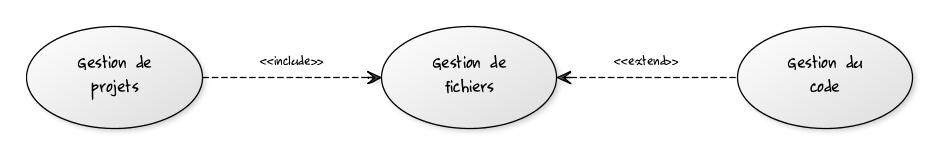
\includegraphics[width=17cm]{images/decompositionSousSystemes.jpg}
					\caption{Décomposition en sous systèmes}
					\label{poulpe}
				\end{center}
			\end{figure}~\\
			Le système de gestion des fichiers est un système très important de l'application et c'est pourquoi il est requis
			par le système de gestion des projets (flèche \emph{include}).\\
			Le système de gestion du code est vue comme une extension aux fichiers. En effet, il serait possible d'éditer un
			site web sans gérer la coloration, l'indentation et toutes les fonctionnalités qui rendent un éditeur de code si agréable à utiliser.
			
			\begin{section}{Gestion des projets}
				Le sous-système de gestion des projets est un élément important de l'application, en ce sens qu'il permet à l'utilisateur
				de bien s'organiser de manière simple et efficace.\\


				À la manière de beaucoup de logiciels connus, il sera nécessaire à l'utilisateur de sélectionner un espace de travail,
				regroupant un ensemble de projets. Cette petite obligation n'est que très peu contraignante et favorise l'organisation, 
				sans pour autant l'imposer réellement à l'utilisateur puisque l'emplacement de cet espace de travail est donné par l'utilisateur.\\


				Un projet est concrètement représenté par un dossier sur la machine de l'utilisateur. Partant de cette idée, notre système
				de gestion de projet sera implémenté en utilisant les normes et références communément admises en termes de création,
				modification et destruction de dossiers.\\


				L'utilisateur doit pouvoir effectuer les actions classiques relatives à un projet, à savoir création, 
				modification, suppression, ouverture et fermeture, il peut également comme stipulé dans le cahier des charges, 
				créer un nouveau projet basé sur un squelette de site pré-existant.\\
				Ce dernier cas de figure, non obligatoire, permet à un utilisateur d'avoir un aperçu de ce que peut être un projet de 
				site internet en développement sous notre application.\\
				L'unique caractéristique d'un projet est que l'on pourra trouver à la racine un fichier spécial résumant les paramètres utilisateur,
				les caractéristiques du projet, et autres informations diverses.\\
				En résumé, concernant les projets, l'application fournit les fonctionnalités décrites dans le diagramme \ref{marchandise}.
				\begin{figure}[ht]
					\begin{center}
						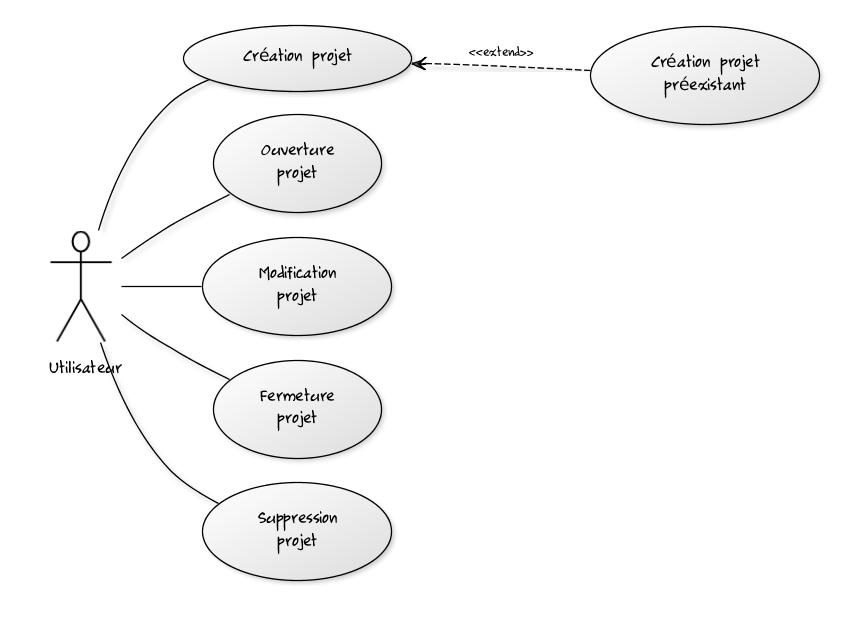
\includegraphics[width=12cm]{images/gestionProjets.jpg}
						\caption{Sous système de gestion des projets}
						\label{marchandise}
					\end{center}
				\end{figure}~\\
				À noter que cette méthode d'utilisation de l'application nous a principalement été inspirée
				par des logiciels que nous utilisons tous en cours et chez nous, comme Eclipse par exemple.\\
				À ces actions d'ordre « général » s'ajoutent quelques actions propres à la modélisation physique des projets dans notre application,
				qui sont exposées dans le diagramme \ref{ucgp}
				\begin{figure}[h]
					\begin{center}
						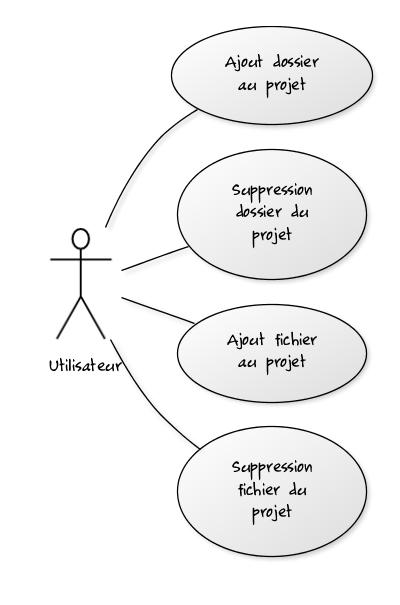
\includegraphics[height=8cm]{images/modificationProjet.jpg}
						\caption{Use-Case modification de projets}
						\label{ucgp}
					\end{center}
				\end{figure}~\\

				Ainsi comme exposé dans ce diagramme, l'utilisateur pourra créer autant de fichiers et de dossiers qu'il le désire dans 
				sont projet, lui permettant ainsi de pouvoir organiser son travail comme il le souhaite, plutôt que devoir se plier à un 
				mode d'organisation imposé par l'application.\\
				Toutefois, ces actions d'apparences basiques sont signes d'un travail important à venir puisqu'elles constituent des libertés
				supplémentaires	accordées à l'utilisateur.\\
			\end{section}
			\begin{section}{Gestion des fichiers}
				Le diagramme \ref{carabine} détaille le contenu du système de gestion des fichiers. Notez l'incroyable similitude entre ce
				dernier et le système de gestion des projets décrits précédemment.\\
				En effet, comme pour les projets, l'application doit permettre d'effectuer des actions basiques en terme de manipulation de fichiers :
				création, ouverture, etc.\\


				L'application jouera cependant un rôle particulier au niveau de l'édition d'un fichier puisque c'est à ce niveau qu'interviendront
				les fonctions de coloration, d'indentation et d'auto-complétion du code, représentées par le système de « gestion du code » dans le 
				diagramme \ref{saphir}. \\
				\begin{figure}[ht]
					\begin{center}
						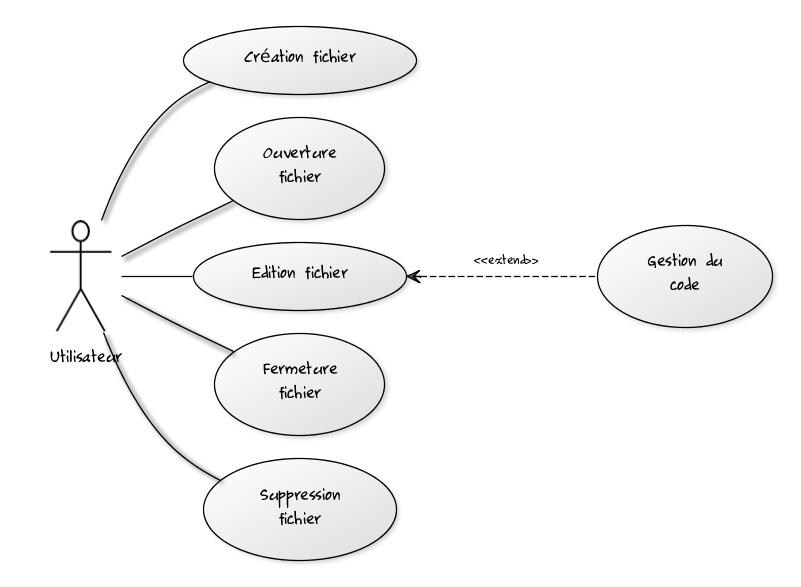
\includegraphics[width=13cm]{images/gestionFichiers.jpg}
						\caption{Sous système de gestion des fichiers}
						\label{carabine}
					\end{center}
				\end{figure}~\\
			\end{section}
			\newpage %% Sinon c'est pas très esthétique.
			\begin{section}{Gestion du code}
				Derrière ce nom quelque peu singulier se cache un concept fort simple, la gestion du code consiste à indenter, colorer,
				visualiser et sublimer le code source présent dans un fichier tel que demandé dans le cahier des charges. Le diagramme \ref{saphir}
				expose les différentes propriétés que doit posséder le système de gestion du code.\\
				L'action étiquetée \emph{Modification du code} correspond à l'édition graphique du texte à l'écran. L'interface graphique
				n'est pas un sous-système en soi du fait notamment qu'elle est incluse dans sous-système de gestion de code.\\
				\begin{figure}[ht]
					\begin{center}
						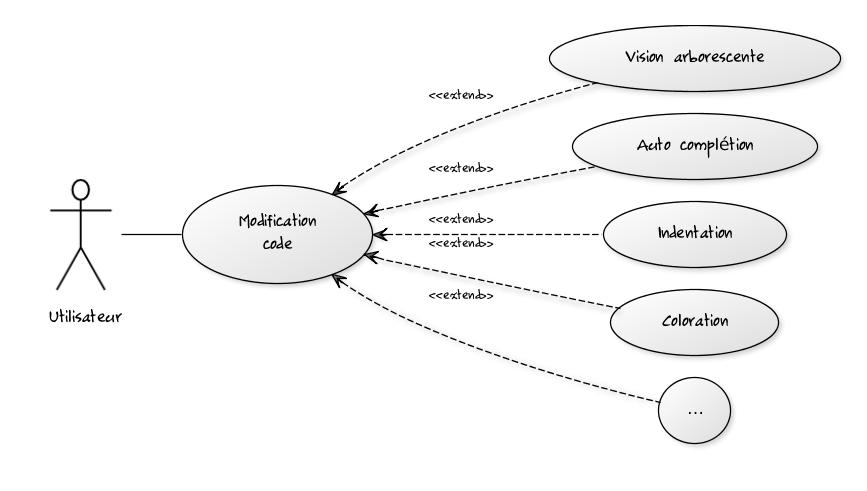
\includegraphics[width=13cm]{images/gestionCode.jpg}
						\caption{Sous système de gestion du code}
						\label{saphir}
					\end{center}
				\end{figure}~\\
			\end{section}
		\end{chapter}
		\begin{chapter}{Diagrammes des classes}
			\begin{section}{Coloration}
				La conception de la partie « coloration syntaxique » de notre application a requis l'introduction de plusieurs classes différentes.
				Tout d'abord des classes dites de données, suffixées du mot anglais \emph{Data}, qui contiennent les différents mots clés relatifs
				à chaque langage sous forme d'\glspl{expression régulière}.\\
				Dans le diagramme \ref{blouson}, nous donnons en exemple une seule classe \emph{HtmlData}, car les autres sont similaires,
				aux particularités du langage près.
				\begin{figure}[ht]
					\begin{center}
						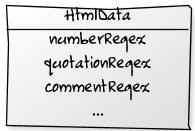
\includegraphics[width=4cm]{images/classesColorationData.jpg}
						\caption{Classe de données pour le langage Html}
						\label{blouson}
					\end{center}
				\end{figure}~\\
				De la même manière, on trouve les classes \emph{CssData, PhpData et JavaScriptData}.\\


				Une autre part de la coloration est l'utilisation concrète des classes décrites précédemment. Sur le diagramme \ref{bicyclette} sont
				représentées toutes les classes qui permettent la coloration à l'écran. Elles héritent d'une superclasse
				\emph{Highlighter} qui factorise la méthode \emph{highlightBlock()}, celle-ci, comme son nom l'indique, colore le texte bloc
				par bloc en fonction des règles données dans les classes \emph{Data}.
				\begin{figure}[ht]
					\begin{center}
						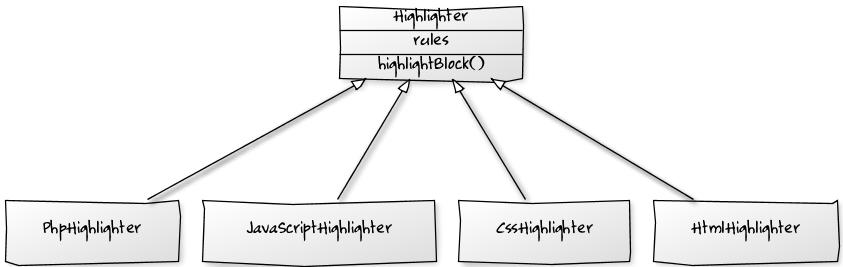
\includegraphics[width=15cm]{images/classesColoration.jpg}
						\caption{Classes de coloration}
						\label{bicyclette}
					\end{center}
				\end{figure}~\\

				Le fonctionnement du module de coloration syntaxique est simple. Une classe est associée à un fichier (voir décomposition de
				l'application, diagramme \ref{poulpe}) selon le code utilisé dans ce fichier. Le texte est analysé grâce aux
				\glspl{expression régulière} des classes de données et les mots reconnus sont formatés dans l'observance des règles édictées dans
				les classes du diagramme \ref{bicyclette}.\\
				Une présentation plus détaillée se trouve dans l'annexe technique à la page \pageref{annexe}.
			\end{section}
			\begin{section}{Système de fichiers}
			\label{classSystem}
				La réflexion autour de l'organisation des fichiers gérés par l'application fût longue, bien que quelque peu avancée par les
				diagrammes de cas d'utilisation que nous avions créés.\\
				En effet, ces derniers nous donnaient un premier aperçu de l'approche à adopter pour traiter le sujet mais nous laissaient quand
				même beaucoup de choix quant au schéma de fichiers à adopter. Notre application suivant bien sûr un développement orienté objet, 
				nous avons eu l'idée de traiter dossiers, projets et espaces de travails comme des instances de classes, pour finalement 
				donner naissance (après quelques essais) au diagramme \ref{arbo}. \\
				\begin{figure}[ht]
					\begin{center}
						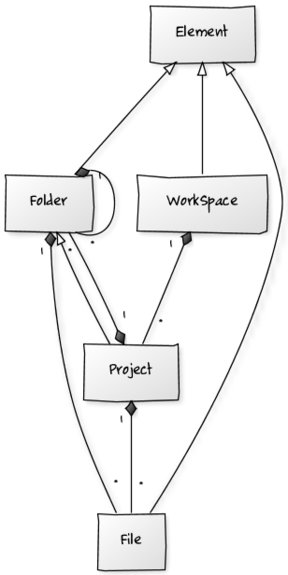
\includegraphics[height=17cm]{images/diagrammeArborescence.png}
						\caption{Classes du système de fichiers}
						\label{arbo}
					\end{center}
				\end{figure}~\\
				Avant d'éditer ce diagramme, nous nous étions mis d'accord, pour des raisons évidentes, sur une factorisation importante de 
				notre code. Ainsi, la classe \emph{Element} regroupe tous les attributs, constantes et méthodes communs à tous les types d'items 
				traités par l'application.\\
				À la manière d'un dossier, un \emph{Projet} pourra être composé de fichiers et de dossiers,
				mais aura des méthodes qui lui sont propres	telles qu'une suppression de son contenu.
				Le \emph{WorkSpace} quant à lui ne sera pas traîté comme un dossier mais plutôt comme un élément particulier ne contenant
				que des projets.\\
				Pour le reste, les classes \emph{Folder} et \emph{File} (resp. \emph{Dossier} et \emph{Fichier}) parlent d'elles-mêmes.
			\end{section}
			\begin{section}{Indentation}
				Nous avons définis avec M. Meynard l'indentation automatique comme étant la capacité qu'a le programme à ajouter (ou retrancher)
				un caractère de tabulation avant une ligne. Nous résolûmes de la mettre en place comme sur le diagramme \ref{guitare}.
				\begin{figure}[ht]
					\begin{center}
						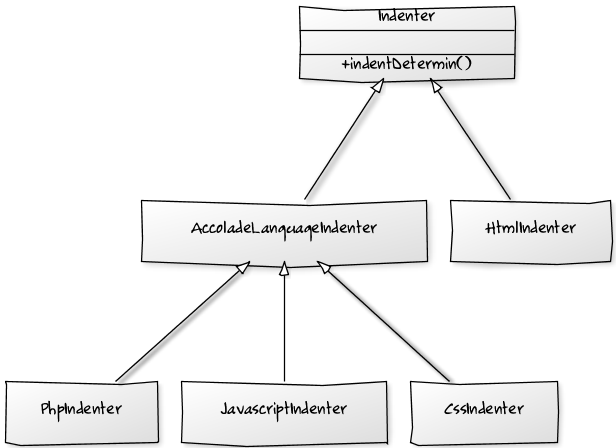
\includegraphics[height=13cm]{images/classesIndentation.png}
						\caption{Classes d'indentation}
						\label{guitare}
					\end{center}
				\end{figure}~\\

				La classe mère \emph{Indenter} est une classe abstraite qui regroupera les méthodes communes à tout indenteur qui se respecte.\\
				Elle est spécialisée par la classe \emph{AccoladeLanguageIndenter} qui, comme son nom l'indique s'occupera de l'indentation des
				langages dont les blocs sont délimités par des accolades, en l'occurence le \gls{Php}, le \gls{JavaScript} et le \gls{Css}.\\
				Ces trois langages possèderont chacun une classe d'indentation spécialisée.\\

				Quant à la classe associée au \gls{Html}, comme celui-ci est langage un peu particulier car il fonctionne par balises, elle
				spécialisera directement la classe \emph{Indenter}.
			\end{section}
			\begin{section}{\Gls{autocomplétion}}
				L'autocomplétion, est une fonctionnalité informatique permettant à l'utilisateur de limiter la quantité d'informations qu'il
				saisit avec son clavier, en se voyant proposer un complément qui pourrait convenir à la chaîne de caractères qu'il a
				commencé à taper.\\
				Dans le	domaine de la programmation où il est souvent besoin de répeter les mêmes instructions et d'écrire les mêmes mots clés,
				cette fonctionnalité est presque vitale.\\


				Il n'existe pas à proprement parler de classe dédiée à l'\gls{autocomplétion} dans notre application.
				En effet, nous intégrâmes directement cette fonctionnalité dans la classe \emph{CentralEditor} par soucis d'optimisation
				et de simplicité.\\

				Différents facteurs entrent en ligne de compte lorsque l'on souhaite parler d'\gls{autocomplétion} :
				\begin{itemize}
					\item l'emplacement du curseur de rédaction ;
					\item le contexte du fichier, c'est-à-dire le(s) langage(s) utilisé(s) dans ce fichier ;
					\item le côté graphique, la visualisation ;
					\item le choix de l'utilisateur d'activer ou de désactiver tel ou tel langage.
				\end{itemize}~\\

				Le diagramme \ref{orangina} représente la classe \emph{CentralEditor} limitée aux attributs et méthodes concernant
				l'\gls{autocomplétion} :
				\begin{figure}[ht]
					\begin{center}
						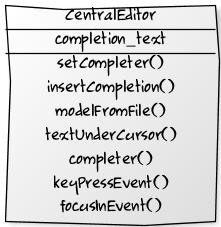
\includegraphics[width=6cm]{images/classesAutoCompletion.jpg}
						\caption{Classe CentralEditor}
						\label{orangina}
					\end{center}
				\end{figure}~\\

				Nous décrirons ici le comportement général des ces méthodes sans entrer dans le détail de chacune d'entre elle,
				ce qui sera fait au chapitre 9.\\

				L'utilisateur commence à taper un mot \emph{m}, l'application ouvre un dictionnaire de donnée correspondant au langage actuel et 
				charge une liste des mots préfixés par \emph{m}. Une fois cette liste construite, elle est affichée à l'utilisateur qui choisit de
				selectionner un mot proposé ou alors de continuer à taper son texte.\\

				Quant aux dictionnaires sus-cités, ils sont au nombre de quatre et contiennent les mots clés de chacun des langages traités (à savoir
				\gls{Html}, \gls{Css}, \gls{JavaScript}, \gls{Php}).
			\end{section}
			\begin{section}{Classes graphiques}
				La partie graphique fût pour nous une nouveauté puisqu'aucun d'entre nous n'avait jusqu'alors participé à un projet d'une si grande
				ampleur avec une interface graphique. Autant dire que les débats furent houleux, chacun ayant sa propre vision des choses.\\
				Et une fois de plus, M. Meynard trancha.\\

				L'interface sera organisée comme sur le diagramme \ref{chauffage}.

				\begin{figure}[ht]
					\begin{center}
						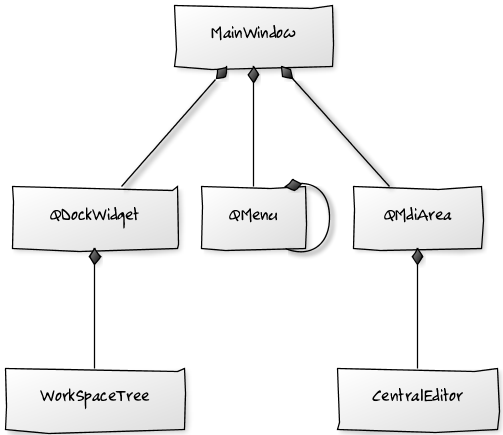
\includegraphics[width=12cm]{images/classesGraphiques.png}
						\caption{Classes de l'interface graphique}
						\label{chauffage}
					\end{center}
				\end{figure}~\\

				Le principe est d'avoir un grand conteneur qui sera la classe \emph{MainWindow}. Ce qui a le double avantage de centraliser
				tout ce qui concerne l'interface au même endroit et de respecter les conventions standard \gls{Qt}.\\


				Toutes les relations présentes dans le diagramme sont des compositions, on observe donc que le \emph{MainWindow}
				(fenêtre principale) est composée de \emph{QDockWidget}, de \emph{QMenu} et d'un \emph{QMdiArea} respectivement
				des barres latérales, des menus et des \gls{MDI} (espaces multidocuments).\\

				On retrouve dans notre barre latérale un \emph{WorkSpaceTree} associé au \emph{WorkSpace} décrit dans la partie \ref{classSystem}
				et qui contiendra une arborescence du ou des projets ouvert(s).\\

				Le \emph{QMenu} sera dédié à des menus classiques avec sous-menus.\\

				Quant au \emph{QMdiArea}, il accueillira un ou plusieurs \emph{CentralEditor}, l'éditeur de texte dans lequel seront appliquées
				toutes les règles de formatages prévues.\\

				Il est bon de préciser que dans le diagramme \ref{chauffage}, les classes dont le nom estpréfixé par la lettre \emph{Q}
				sont des classes de \gls{Qt}, pour les autres, nous en seront les auteurs.
			\end{section}
		\end{chapter}
		\begin{chapter}{Organisation du code : le modèle MVC}

			Avant de réellement commencer la programmation (partie suivante), il nous a fallu parler de la façon dont nous allions organiser
			notre code. \gls{Qt} est conçu pour gérer des projets organisés selon le modèle \gls{MVC}, il était donc logique de se pencher
			sur la question. D'autant plus que ce patron de conception est actuellement très prisé dans le monde de la programmation.\\


			Le \gls{MVC} est donc un modèle de programmation qui repose sur la séparation du code produit en trois grandes catégories
			représentées sur le schéma \ref{sinistre}.\\
			\begin{figure}[ht]
					\begin{center}
						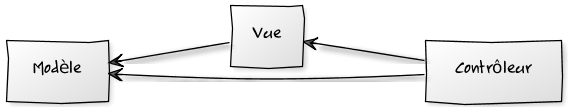
\includegraphics[width=9cm]{images/mvc.png}
						\caption{Les trois catégories du MVC}
						\label{sinistre}
					\end{center}
				\end{figure}~\\


			\begin{description}
				\item[Le modèle :] représente tous les aspects du comportement de l'application, c'est-à-dire le traitement des données
				et toutes les interactions avec une éventuelle base de données, c'est lui-même qui décrit toutes les données et qui 
				définit comment l'application va accéder et intéragir avec ces dernières.
				\item[La vue :] l'interface sur laquelle va agir l'utilisateur, c'est elle qui se charge de présenter les données
				renvoyées par le modèle, de les afficher, et éventuellement de donner la possibilité à l'utilisateur d'interagir sur 
				ces dernières, mais la vue n'effectue aucun traitement, son travail ne consiste qu'en la présentation des données, 
				en aucun cas elle ne doit effectuer de traitement direct sur des données. Dans certains environnements, elle est écrite 
				grâce à des langages de présentation uniquement (comme \gls{Html} et \gls{Css}), ce qui permet de la limiter à sa fonction première.
				\item[Le contrôleur :] Il est l'agent de réponse à un utilisateur. Généralement, lui non plus n'effectue pas de traitement,
				mais se charge d'analyser chaque requête de l'utilisateur, chacune de ses interactions avec la vue, et il fera appel
				au modèle et à la vue qui conviennent à chacune de ces requêtes. Le contrôleur est un peu l'interprète de l'utilisateur,
				c'est lui qui va comprendre qui concerne la requête souhaitée, appeler le modèle correspondant, et renvoyer une vue
				liée à la demande.
			\end{description}

		\end{chapter}
	\end{part}
%%%%%%%%%%%%%%%%%%%%%%%%%%%%%%%%%%%%%%%%
%%%%%%%%%%%%%%%%%%%%%%%%%%%%%%%%%%%%%%%%
	\begin{part}{L'oeuvre}
		\begin{chapter}{Travail de groupe}
			\begin{section}{Répartition des tâches}
				C'est une fois la conception terminée que se fit sentir le besoin de distinguer différentes parties dans le projet. Ceci afin de
				marcher fermement dans un sens bien défini et d'éviter des erreurs de planification.
				Nous sollicitâmes donc quelques conseils auprès de M. Meynard qui nous aida donc à déterminer les grandes parties qui pouvaient 
				être séparées. C'est ainsi que virent le jour trois orientations :\\
				\begin{description}
					\item[Interface :] tout ce qui se voit à l'écran tels fenêtres, onglets, menus et autres.
					\item[Système :] fonctionnalités qui touchent au système de fichier comme la gestion des fichiers ou d'un espace de travail.
					\item[Fonctions :] fonctionnalités de gestion du code comme le sont la coloration, l'indentation ou l'\gls{autocomplétion}
				\end{description}~\\


				Il est judicieux lorsqu'un projet est fractionné comme l'est le nôtre, de constituer autant de groupes que de parts de travail.\\
				En vertu de ce principe, nous décidâmes de constituer trois groupes constitués comme suit :\\

				\begin{itemize}
					\item Groupe \emph{interface} : Hamza, Issame et Zaydane ;
					\item Groupe \emph{système} : Mickael et Joachim ;
					\item Groupe \emph{fonctionnalités} : Pierre, Olivier et Abdelhamid.
				\end{itemize}~\\

				Il est arrivé bien des fois qu'un groupe rencontre un problème ardu ne pouvant être surmonté sans aide extérieure.
				Heureusement pour lui, les deux autres étaient là pour lui prêter main forte. Ainsi fûrent maintenues tout au long de notre travail
				une grande cohérence et une grande adéquation relativement à l'évolution des différentes parties.\\


				Néanmoins, les membres du groupe étant d'horizons estudiantins différents (comprenez par là qu'ils ne besognent pas pareillement),
				il s'avéra nécessaire d'édicter différentes normes quant aux méthodes de travail à adopter.

			\end{section}
			\begin{section}{Conventions techniques}
				Voici une liste des conventions prises pour la programmation, les commentaires du code source et le nommage des fichiers.
				%% Petite note de bas de page.
				\addtocounter{footnote}{2}
				\footnotetext[\value{footnote}]{Le nom de fonction désigne aussi les méthodes.}
				\begin{itemize}
					\item Les noms de classes, structures, fonctions$^{\decimal{footnote}}$, variables et constantes seront donnés en anglais.
					\item Les noms de fonctions et variables commencent par une minuscule (une minuscule en anglais bien sûr).
					\item Les noms de classes et structures commencent par une majuscule.
					\item Les noms de constantes s'écrivent avec uniquement des majuscules et des tirets bas (le fameux trait du 8).
					\item Les noms de fichiers qui déclarent et définissent une classe (.h et .cpp) portent le même nom que la classe, avec la
					majuscule.
					\item Les noms de fichiers normaux commencent par une minuscule (p.ex. main.cpp).
					\item L'indentation est laissée libre (accolade en fin de ligne ou en ligne suivante) pour n'embarrasser personne et ne pas
					créer de controverse.
					\item Toute classe, fonction ou structure sera bien commentée en utilisant la notation \gls{Doxygen}.
					\item Dans une moindre mesure, il sera possible de commenter les variables et constantes importantes avec la même notation.
				\end{itemize}~\\

				Bien que les règles citées ci-dessus soient des conventions communément admises (dans le monde \gls{C++} du moins), il valait mieux
				bien les préciser de manière à éviter toute mauvaise surprise.
			\end{section}
			\begin{section}{Les réunions hebdomadaires}
				Le grand chamane de l'UM2 a prévu dans notre emploi du temps un créneau d'une heure trente le lundi et le mardi intitulé « Projet ».
				Étant par nature opportunistes, nous tînmes nos conseils de projet précisément durant ces créneaux.\\


				Une réunion de projet se déroule toujours de la même manière. Chacun des trois groupes résume le travail effectué durant la semaine,
				fait part de ses problèmes éventuels et donne la liste des choses prévues pour la semaine d'après.
				S'ensuit une séance de remue-méninges pour discuter, critiquer, approuver ou réprouver ce qui vient d'être présenté.
				Parfois, des discussions moins techniques venaient nourrir le débat, relatives par exemple à l'organisation de ce document.\\

				Il existe un rapport de chacune de ces réunions, sous la forme d'un site créé par les soins d'un membre du groupe.
				Après chaque colloque, notre scribe désigné se chargeait de résumer la session afin de garder une trace datée et titrée qui
				servirait de journal de bord.

				\begin{figure}[ht]
					\begin{center}
						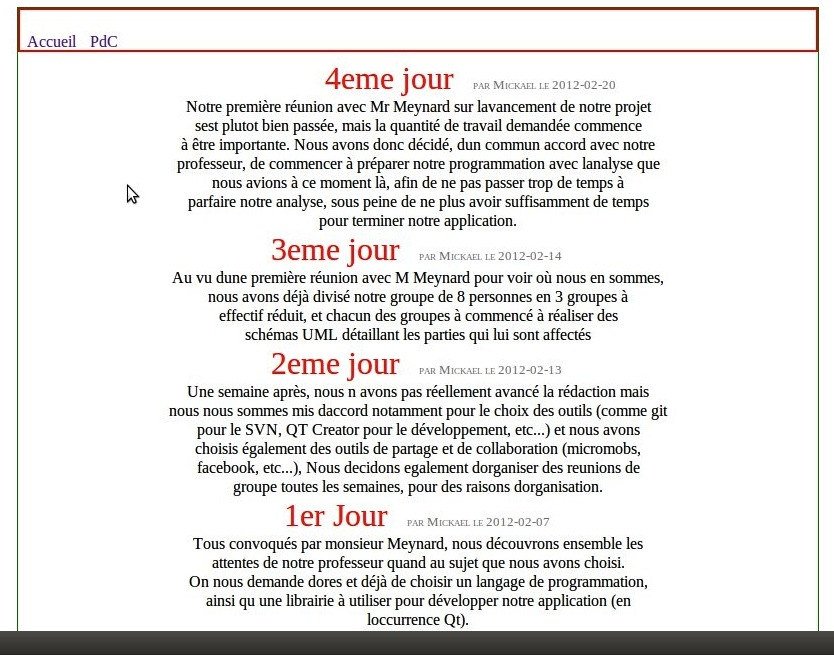
\includegraphics[width=18cm]{images/journal.jpg}
						\caption{Un extrait du journal de bord}
					\end{center}
				\end{figure}~\\

			\end{section}
		\end{chapter}
		\begin{chapter}{Implémentation}
			\begin{section}{Arborescence du projet}
				Le projet est organisé comme sur l'arborescence \ref{dindon}. On dispose à la racine du projet de trois sous-dossiers correspondants
				aux trois éléments du \gls{MVC}. Chaque fichier source créé trouve sa place de manière évidente dans cette arborescence.\\
				Par exemple, pour qui cherche le fichier \emph{WorkspaceTree.cpp}, il est manifeste que celui-ci se situe dans le dossier \emph{View}.
				\\
				De même que le fichier \emph{CSSData} qui décrit des données, sera dans le dossier \emph{Model}.\\
				Cette distribution nous mis à l'abri de beaucoup de problèmes qui adviennent dans un travail de groupe, comme la suppression
				accidentelle ou le sabotage du travail d'autrui.\\

				\begin{figure}[h]
					\begin{center}
						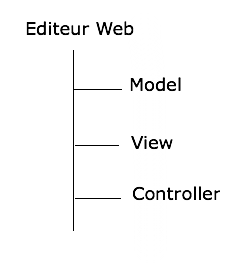
\includegraphics[width=7cm]{images/arborescenceProjet.png}
						\caption{Arborescence de projet}
						\label{dindon}
					\end{center}
				\end{figure}~\\
			\end{section}
			\begin{section}{Système}
			\label{calebasse}
				Arrivés au stade de l'implémentation système, nous avions une idée relativement fixe de l'organisation des fichiers servant au
				développement de l'aspect \emph{système} de l'application. Nous savions également ce qu'allait donner visuellement notre travail
				à savoir une arborescence de fichiers sur la gauche de la fenêtre principale, à la manière d'un Eclipse ou d'un QT Creator.
				L'envie de commencer à programmer se faisait plus que jamais ressentir, mais quelques petits détails restaient encore à régler.\\


				En effet, l'utilisation de \gls{Qt} ainsi que de l'architecture \gls{MVC} nous contraint à nous documenter sur ce que ce 
				framework proposait pour répondre à nos attentes.\\
				La réponse ne tarda point puisque le \emph{QDirModel} apparaissait comme correspondant parfaitemement, étant donné qu'il s'agit d'un
				modèle de données spécialement conçu pour être peuplé par une arborescence de fichiers.\\


				Malheureusement, cette solution s'est rapidement montrée insuffisante pour ce que nous prévoyions, notamment à cause du fichier de 
				configuration de nos projets. Notre idée étant de remplir l'arborescence d'espace de travail de l'utilisateur uniquement par des
				projets, qui, comme expliqué plus haut, sont des dossiers contenant un fichier de configuration nommé \emph{.pro} à leur racine.\\
				Le \emph{QDirModel} ne permet pas de filtrer la population du modèle selon un quelconque paramètre donc a fortiori le paramètre
				d'existence d'un éventuel \emph{.pro}.

				Nous arrêtâmes de créer nous même des fonctions remplissant notre modèle de données selon le type de l'élément rencontré
				(\emph{WorkSpace}, \emph{Project} ou \emph{Folder}). Ce qui permettait non seulement de filtrer le remplissage des modèles mais
				également d'effectuer certaines actions directement lors du parcours (récursif) de l'arborescence de fichiers.
				Par exemple attribuer des noms aux éléments trouvés, instancier des objets correspondant aux éléments (\emph{File}, \emph{Folder},
				\emph{Project}) et bien d'autres choses.\\


				Ces fonctions (nommées \emph{scan} dans les classes), consistent en des parcours récursifs de l'arborescence \emph{WorkSpace}.
				La difficulté réside dans la cohabitation de nos classes avec celles du \gls{C++}.\\
				Outre quelques initialisations de structures (\emph{Dirent}, \emph{Dir}, \emph{stat}, ...) et variables de parcours, il faut des
				conversions des chemins de fichiers de type \emph{string} vers le type \emph{char*} pour correspondre aux signatures de certaines
				fonction de \gls{C++}.


				Si l'ouverture ne pose pas de problèmes, la ligne \mint{cpp}|folderPath = (char*)malloc(folderPathSize * sizeof(char));|
				alloue la mémoire nécessaire pour le parcours.\\
				Cette ligne d'apparence ordinaire mérite d'être soulignée puisqu'elle fait partie de celles qui ont engendré des problèmes de fuites
				mémoire, dont la résolution fut longe et pénible.\\


				L'intérêt de créer notre propre fonction de scan commence d'ailleurs par cette ligne, puisque chaque élément de l'arborescence qui
				sera ajouté au modèle se voit instancié et affecté d'un attribut \emph{path}, une chaine de caractère permettant de stocker le chemin
				(relatif à la racine de l'arborescence) du fichier qu'il représente.
				S'ensuit un léger jeu de concaténations pour éventuellement créer le chemin d'un fichier de configuration \emph{.pro}, qui s'il est
				trouvé augmentera la liste des projets gérés.\\


				Une fois le workspace choisi, une vue interactive sur l'arborescence des projets est disponible.\\
				Le double clic entraîne l'ouverture du fichier ou l'ouverture/fermeture d'un dossier/projet.
				Le clic droit quand à lui ouvre un menu déroulant, dans lequel on retrouve les options classiques : déplacement, copie, renommage, ouverture, suppression, ajout de fichier, de dossier, et caetera.\\

				\begin{figure}[h]
					\begin{center}
						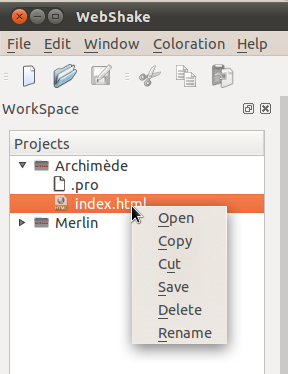
\includegraphics[width=8cm]{images/interactions.png}
						\caption{Les options disponibles au clic droit}
						\label{flute}
					\end{center}
				\end{figure}~\\
			\end{section}
			\begin{section}{Fonctionnalités}
				\begin{subsection}{Coloration}
					La coloration est un principe simple et rapide en mettre en oeuvre, ce fut la première fonctionnalité à être implémentée.\\
					Le principal problème est de gérer une coloration sur plusieurs lignes étant donné que l'analyse du texte se fait ligne par
					ligne.\\

					La solution fut de créer des états tels que \emph{IN_COMMENT_STATE} par exemple, qui permettent de savoir si la ligne courante
					est en commentaire ou non.
					\begin{figure}[h]
						\begin{center}
							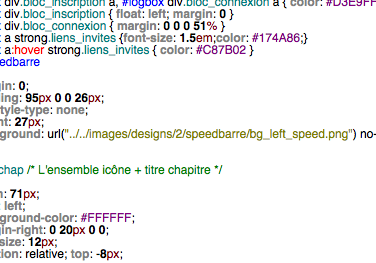
\includegraphics[width=8cm]{images/screenColoration.png}
							\caption{La coloration en action}
						\end{center}
					\end{figure}~\\					
				\end{subsection}
				\begin{subsection}{\Gls{autocomplétion}}
				\label{autocompl}
					La mise en place du système d'autocomplétion n'a pas posé de problèmes principalement parce qu'il est inspiré d'un exemple de
					la documentation.\\

					%% Petite note de bas de page.
					\addtocounter{footnote}{3}
					\footnotetext[\value{footnote}]{le bloc désigne un morceau de code inclus dans un autre morceau de code.}
					Le principal problème fut de gérer une \gls{autocomplétion} contextuelle de bloc$^{\decimal{footnote}}$
					et force est de constater que la tâche n'est pas tout à fait achevée.\\
					Pour réaliser une telle prestation, il est nécessaire que notre application puisse faire l'analyse
					grammaticale du code source. Or aucun analyseur syntaxique (\gls{parseur}) n'est inclus dans le programme ce qui empêche
					un fonctionnement optimal de cette fonctionnalité.\\


					Néanmoins nous avons pu ruser et essayer de deviner le bloc courant en fonction des lignes qui précèdent celle où se
					trouve le curseur. Par exemple, une ligne qui se trouve après une autre ligne qui contient l'expression \emph{<script>}
					dans un code \gls{Html}, sera autocomplétée avec le dictionnaire du \gls{JavaScript}.\\
					Cette stratégie trouve rapidement ses limites, par exemple si une balise fermante \emph{</script>} se trouve en début
					de ligne.\\


					La figure \ref{tabouret} représente le module d'\gls{autocomplétion} en pleine action dans le contexte du langage \gls{Php}.

					\begin{figure}[h]
						\begin{center}
							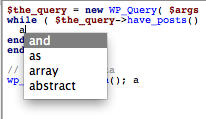
\includegraphics[width=6cm]{images/screenAutocmpl.png}
							\caption{L'autocomplétion en pratique}
							\label{tabouret}
						\end{center}
					\end{figure}~\\
				\end{subsection}
				\begin{subsection}{Indentation}
					L'implémentation de ce module ne fut pas une mince affaire, car qui veut indenter un morceau de code passe 
					de préférence par une arborescence représentative dudit code. Ce qui nécessite la mise en place d'un \gls{parseur}.\\
					Après nous être renseignés, notamment auprès de M. Meynard, nous prîme la décision de créer un analyseur basique. 
					Celui-ci se chargera de lire le code, d'en extraire des mots importants (avec des \glspl{expression régulière})
					et de décider en fonction de deux paramètres le niveau d'indentation de la ligne courante.\\
					Ces paramètres sont:
					\begin{itemize}
						\item La profondeur d'indentation de la ligne précédente ;
						\item La présence ou non de caractère spéciaux dans la ligne précédente (par exemple l'accolade ouvrante) ;
					\end{itemize}~\\

					Dès lors la fonction d'indentation ne fut plus qu'une formalité si l'on néglige les quelques heures à traquer les erreurs
					telles que balise ouvrante et fermante sur la même ligne par exemple.

					\begin{figure}[h]
						\begin{center}
							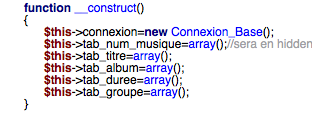
\includegraphics[width=6cm]{images/indentBien.png}
							\caption{Un code bien indenté par l'application}
						\end{center}
					\end{figure}~\\
				\end{subsection}
			\end{section}
			\begin{section}{Interface}
				Le principal inconvénient concernant la mise en oeuvre de l'interface fut l'apprentissage de la documentation.\\
				Il fallait non seulement comprendre les concepts de programmation d'interface graphique mais en même temps mettre
				en application lesdits concepts.\\

				Nous rencontrâmes donc plusieurs problèmes de synchronisation car les différents membres du groupe n'étaient pas toujours
				d'accord sur des détails techniques.\\

				Finalement, les trois personnes chargées de l'interface conçurent un modèle simple basé sur la stratégie de l'éparpillement.\\
				Chaque élément de l'interface est séparé des autres dans une classe spécialisée avant d'être regroupés dans la \emph{MainWindow}.\\

				Il est possible d'admirer le résultat du travail du groupe \emph{Interface} dans le chapitre suivant.
			\end{section}
		\end{chapter}
		\begin{chapter}{Résultat}
			Le meilleur moyen de faire le bilan de ces trois mois de travail est de comparer les résultats obtenus avec le cahier des charges initial.\\
			Mais avant cela, jetons un regard sur le côté graphique de l'application.\\

			Dès l'ouverture de l'application, l'utilisateur peut voir sur son écran là même chose que sur la figure \ref{mayonnaise}.

			\begin{figure}[h]
				\begin{center}
					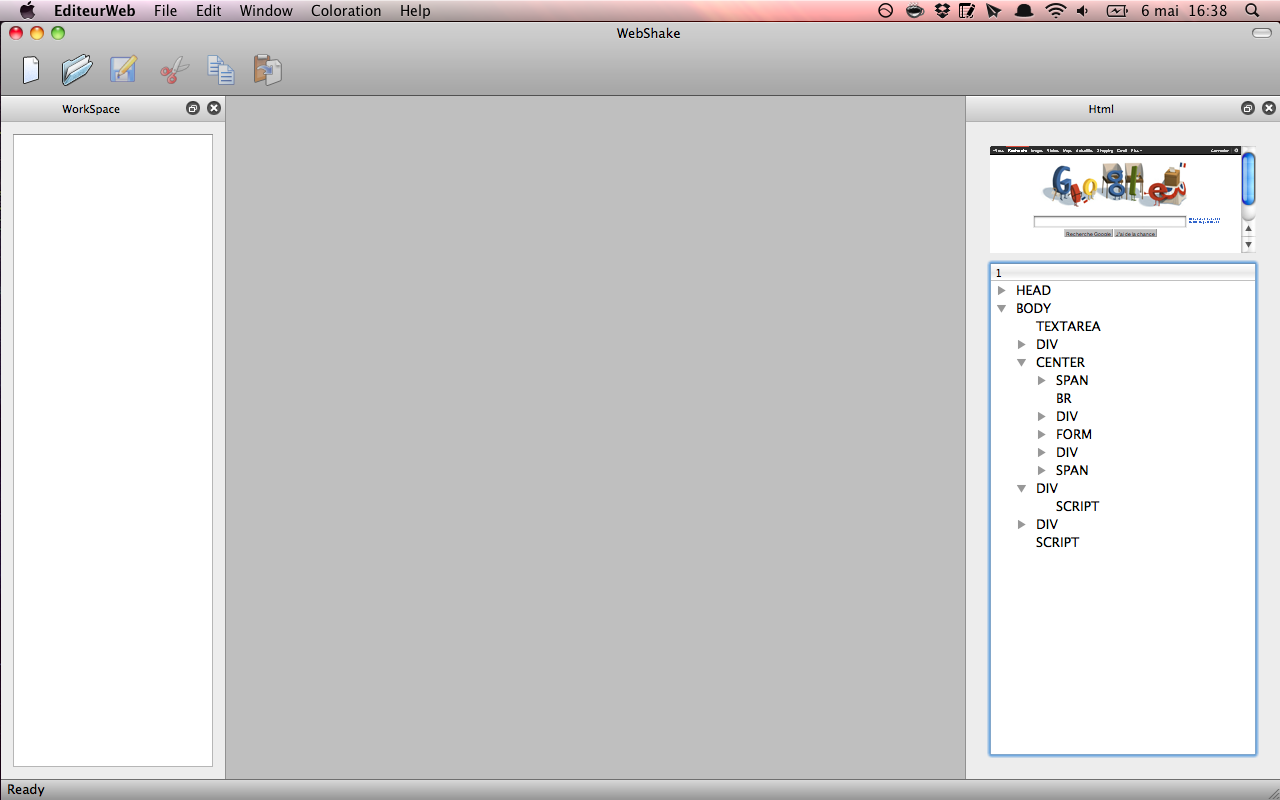
\includegraphics[width=15cm]{images/screenOpening.png}
					\caption{L'écran à l'ouverture de l'application}
					\label{mayonnaise}
				\end{center}
			\end{figure}~\\


			On aperçoit différents éléments classiques comme la barre de menus par exemple et les trois inévitables boutons des coins de fenêtre qui sont fermer, réduire ou agrandir. Le bandeau d'actions donne à l'utilisateur le pouvoir d'ouvrir ou d'enregistrer, de copier ou de coller
			à sa guise.\\


			À gauche, se trouve un espace vide pour l'instant mais qui va bientôt accueillir l'arborescence du projet que l'utilisateur
			s'apprête à créer ou à ouvrir, cet espace incarne le fameux \emph{workspace}, oeuvre du groupe \emph{système}.\\


			La grande région grisâtre au centre de l'écran va recevoir un (ou plusieurs) éditeur de texte spécialisé dans l'un des langages
			\gls{Html}, \gls{Css}, \gls{Php} ou \gls{JavaScript}. C'est ici que prennent forme les heures de dur labeur du groupe
			\emph{fonctionnalités}.\\


			Enfin, la partie de droite est une idée du groupe qui n'était pas dans le cahier des charges. Cet espace semblait vide, inerte et désolé.
			Alors nous eûmes l'idée d'en faire un emplacement de visualisation. Entendez par là un emplacement dédié au programmeur, pour qu'il
			voie en direct les effets de ce qu'il est en train d'écrire.\\
			La partie haute est un aperçu sur navigateur du site en cours d'édition et la partie basse une arborescence de l'inclusion des
			différents blocs de code.\\
			Malheureusement cette fonctionnalité n'a pas abouti du fait notamment qu'il faut \gls{parseur} pour générer une arborescence.\\


			Dans le tableau \ref{raisin}, sont rassemblées toutes les spécifications du cahier des charges (colonne de droite) et il est
			précisé si notre application possède ou non ces propriétés.\\
			\begin{table}[h]
			\caption{\label{raisin} Comparatif avec le cahier des charges}
			\centering
				\begin{tabular}{|c||c|} % c signifie center, le texte de chaque colonne sera donc centré.
				  \hline
				  Fonctionnalité & présente ? \\
				  \hline
				  Édition de fichiers dans quatre langages & oui \\
				  Système multi-onglets & oui \\
				  Arborescence du site & oui \\
				  Autocomplétion & oui \\
				  Coloration syntaxique & oui \\
				  Indentation automatique & oui \\
				  Accès aux manuels & non \\
				  Validation \gls{Html} & non \\
				  Visualisation du site & oui \\
				  Squelette de site préexistant & non \\
				  \hline
				\end{tabular}
			\end{table}~\\

			Malgré le fait que le cahier des charges soit presque complété, il subsiste dans les parties achevés quelques \glspl{bogue} épars
			dont nous discuterons dans le chapitre suivant.
		\end{chapter}
		\begin{chapter}{Discussion}
			\begin{section}{Cahier des charges}
				Comme on peut le constater sur le tableau précédent (\ref{raisin}), le cahier des charges est presque complété.
				Il reste néanmoins l'accès aux manuels,	la validation \gls{Html} et des sites préfabriqués.\\
				À notre décharge, nous pouvons arguer que ces fonctionnalités ne nous ont pas posé de problème technique mais plutôt organisationnel.
				En effet, si l'on regarde le diagramme de Gantt de la page \pageref{flute}, on remarque que nous nous apprêtions à travailler
				jusqu'à la fin du mois de mai ce qui nous aurait laissé le temps de terminer ces modules très simples à mettre en place.\\


				Si l'on juge du point de vue quelque peu pragrmatique, on pourra constater quelques manques à l'application.
				Citons une fois de plus le \gls{parseur} qui aurait dû être la base de l'application mais dont la réalisation demandait
				un temps trop considérable au vu de	celui qui nous était imparti.\\
				Fut donc réalisé, avec astuce et stratagème, un « pseudo-parseur » réalisant l'analyse syntaxique à la volée. Cette analyse ne génère
				pas d'arborescence comme il se devrait et voilà le problème, c'est que celle-ci est indispensable au bon fonctionnement de certains
				module comme l'\gls{autocomplétion} contextuelle (cf. page \pageref{autocompl}).\\
			\end{section}

			\begin{section}{Considération graphique}
				L'application utilise les éléments graphiques du système dans lequel elle est utilisée. Elle n'est donc pas réellement personnalisée
				et ne possède pas d'identité graphique propre (mis à part les icônes).\\
				Ce manque de charisme, cette sobriété diraient certains, n'influent que très peu sur l'impact réel provoqué sur l'utilisateur.
				Celui-ci étant un programmeur il est certainement habitué à d'horribles interfaces de programmation voire de ligne de commandes.\\


				Aucune instruction ne nous ayant été donnée quant à la réalisation de cette interface, elle est entièrement de notre cru et
				nous sommes satisfait du résultat.
			\end{section}

			\begin{section}{Aller plus loin}
				L'application est perfectible à bien des égards, les fonctionnalités principales sont présentes mais nous pourrions tout aussi
				bien ajouter :
				\begin{itemize}
					\item Une fonctionnalité de glisser déposer pour gérer les fichiers intuitivement dans le panneau gauche.
					\item Différentes palettes de couleurs pour la coloration syntaxique.
					\item Un \emph{WorkSpace} par défaut.
					\item Un mode de formatage d'un fichier mal indenté.
				\end{itemize}~\\

				De même, il est possible d'ajouter des éléments graphiques pertinents, comme un panneau proposant la documentation du langage
				actuellement utilisé.\\
			\end{section}
		\end{chapter}
	\end{part}
%%%%%%%%%%%%%%%%%%%%%%%%%%%%%%%%%%%%%%%%
%%%%%%%%%%%%%%%%%%%%%%%%%%%%%%%%%%%%%%%%
	\begin{chapter}*{Conclusion}
	\addcontentsline{toc}{chapter}{Conclusion}
		Pour faire le bilan de ce projet, rien de tel que donner à chaque membre du groupe quelques lignes pour s'exprimer.

		\begin{section}*{Pierre}
Pour ma part, ces 3 mois de travail ont été une grande source d'apprentissage. J'ai découvert une nouvelle façon de travailler,
		grâce à l'utilisation d'un gestionnaire de version tel que GitHub. Réaliser un projet regroupant 8 personnes était également une grande première.
		Ceci a pu nous donner un aperçu des inconvénients et des avantages de réaliser un logiciel en grand nombre. Difficultés de communication,
		de synchronisation, de partage des tâches. . . Cependant, cette expérience a surtout été bénéfique. Apprendre à dialoguer, s'entraider, échanger ses
		idées et débattre autour des stratégies à adopter a été très enrichissant. Enfin, la découverte du framework QTCreator m'a énormément plu.
		Relativement intuitif et assez rapide à prendre en main, il offre un confort non négligeable dans la programmation,
	    avec des librairies très nombreuses et très utiles.\\
	    En somme, la tâche qui nous a été confiée m'a appris énormément de choses, que ce soit dans le domaine de la programmation pure ou dans les 
	    relations entre tous les membres d'un groupe.
		\end{section}

		\begin{section}*{Olivier}
		Tout au long de ces trois mois, il n'y avait pas une seule semaine qui apportait sa nouveauté. L'initiation
à un système de gestion de version tel que GitHub, l’apparition d'un nouvel environnement de développement avec QtCreator (et ses nombreuses librairies, sa documentation touffue), la direction d'un groupe de huit personnes, toutes ces choses ont été nouvelles pour moi.\\
Concernant la gestion du groupe, il m'a fallu être démocratique, laisser fleurir les idées en vrac, canaliser chaque esprit vers notre objectif. Il a fallu parfois prendre des décisions difficiles rapidement, tout en respectant les opinions de chacun. Occasionnellement, il a fallu également forcer le destin et s'imposer dans les moments difficiles.\\
Pour ce qui est de la programmation le MVC m'a permis de ne pas me disperser, de respecter une standardisation connue. L'utilisation d'un nouveau framework , et l'utilisation de sa documentation a été forcément pour moi une nouveauté. Ce dernier m'a réellement plu pour son utilisation simpliste, épurer ... bref tous les avantages d'un IDE.\\
Ce projet m'a également ouvert les yeux sur l'ampleur de la prise en main d'un tel projet. Proche d'un logiciel commercial, ce dernier m'a encouragé à persévérer dans mes convictions et dans la concrétisation sous mes yeux d'un projet d'importance.\\ 
Ce projet m'a beaucoup plu. Il m'a apporté toutes les expériences proches de celles des entreprises. Tant au point de vu collaboration concernant le groupe, et tout autant au point de vu apprentissage et prise en main de nouveaux outils très pratique pour la situation à laquelle nous étions confrontés.\\
		\end{section}

		\begin{section}*{Hamza}
		\end{section}

		\begin{section}*{Issame}
		\end{section}

		\begin{section}*{Mickaël}
		Bien qu'au départ, l'idée de travailler en groupe à grand effectif sur un projet m'effrayait quelque peu, c'est finalement un des aspects de notre 		   projet qui m'a le plus plu.
		En dehors de mon enrichissement personnel à travers l'apprentissage de nouveaux outils tels que Qt, Doxygen ou même juste certains aspects du
		langage C++ que je ne connaissais pas encore, c'est dans l'utilisation des plateformes et outils de collaboration comme git, micromobs ou yUML
		que j'ai le plus trouvé mon bonheur. En effet, bien plus qu'une simple application réalisée à plusieurs, ce projet a été pour moi un aperçu
		important de ce que peut être un travail en équipe dans une entreprise, et de ses nombreux aspects d'organisation, de la tenue d'un journal de
		bord aux réunions obligatoires toutes les semaines, en passant par la communication très importante sur ce que l'on est ou que l'on va faire
		concernant le projet (afin d'éviter toute confusion),qui sont pour moi des situations auxquelles il est plus que bon d'avoir déjà fait face
		avant un premier emploi dans le domaine.\\
		De mon point de vue, ce projet s'est donc montré plus qu'édifiant, et a surtout renforcé ma motivation pour l'avenir.\\
		\end{section}

		\begin{section}*{Joachim}
		Ma conclusion: Pour ma part le projet fût une bonne expérience, premièrement il m'a permit de développer mes compétences dans le language c++, apprendre à utiliser Qt et tout un tas d'outils jamais utilisé jusqu'alors: Valgrind, Git, yUml, etc.
Deuxièmement, ayant déjà réalisé un projet à l'IUT, il ne m'était jamais arrivé de travailler avec autant de personne. Celà fût fort agréable, car en ayant réussi à diviser notre projet en sous parties, on voyait vraiment que chacun des groupes apportait sa pierre à l'édifice tout en restant cohérent sur le résultat final.
Pour finir je dirais que le projet nous permet à chacun de nous de toucher du doigt notre futur travail, ce qui est vraiment motivant.
J'ai lu le rapport hier, j'ai souligné quelques fautes par ci par là, tu voudras que je te les montre?
		\end{section}

		\begin{section}*{Zaydane}
		\end{section}

		\begin{section}*{Abdelhamid}
		\end{section}

		Ainsi s'achève ce document (en fait non, il y a encore une annexe après).\\
	\end{chapter}
%%%%%%%%%%%%%%%%%%%%%%%%%%%%%%%%%%%%%%%%
%%%%%%%%%%%%%%%%%%%%%%%%%%%%%%%%%%%%%%%%
	\begin{chapter}*{Annexe technique}
	\label{annexe}
	\addcontentsline{toc}{chapter}{Annexe technique}
	\begin{section}{À propos de Qt}
			Travailler avec \gls{Qt}, c'est travailler avec un immense ensemble de classes diverses et variées. 
			Il y a des classes graphiques, des classes pour le XML, des classes pour le son, des classes pour tout ce qu'une application classique
			peut nécessiter pour fonctionner.\\

			Cet état des choses peut sembler idéal de prime abord, amenant rapidement à des énoncés tels que « Facile, il suffit de prendre telle classe
			et de l'utiliser. » ou bien « Ah beh je vais employer cette classe elle fait ça très bien. ». Néanmoins, prendre l'habitude de ce genre de 
			discours conduit à la paresse du programmeur qui fournira une application avec des fonctionnalités réduites,
			limitées par la classe de \gls{Qt}.\\

			De plus, construire soit même une ensemble de classe en dehors de \gls{Qt} est très difficile. Au vu du grand nombre de classe qui
			accomplissent telle ou telle tâche, on se sent obligé de les utiliser. D'autant plus que la documentation nous y encourage en donnant des exemples de codes orientés \gls{Qt}, transformant de ce fait \gls{Qt} en élément du langage.\\

			\noindent
			Par exemple, au lieu d'écrire ce code : 
			\begin{center}
			\begin{cppcode}
std::string avertissement = "Holà ! cavalier, vous voyagez sans selle !";
std::vector<int> v;
			\end{cppcode}
			\end{center}
			Il est conseillé d'écrire : 
			\begin{center}
			\begin{cppcode}
QString avertissement = "Holà ! cavalier, vous voyagez sans selle !";
QVector<int> v;
			\end{cppcode}
			\end{center}~\\

			Il est donc presque impossible, si l'on suit cette philosophie, de créer une classe que l'on va utiliser dans un projet \gls{Qt} et 
			ensuite récupérer dans un autre projet sans faire de modification.\\

			Au contraire, à qui sait bien l'utiliser \gls{Qt} est une véritable merveille.\\
			Ci-après, le code de la classe JavaScriptHighligher qui regroupe les différents formats associés à des mots du langage.
			Grâce à l'utilisation pertinente des classes \emph{QSyntaxHighlighter} (dont hérite la classe Highlighter) ou \emph{QRegex}, on peut
			réduire un colorateur syntaxique complet à ces quelques lignes de code.\\

			La méthode \emph{addRule} ajoute une nouvelle règle de coloration au colorateur tandis que le attributs dont le nom termine par
			\emph{Format} sont de type \emph{QTextCharFormat}, une classe qui définit des règles de formatage de texte.
			\begin{center}
			\begin{cppcode}
#include "JavaScriptHighlighter.h"

JavaScriptHighlighter::JavaScriptHighlighter(QTextDocument *parent)
: Highlighter(parent)
{
    // Les nombres.
    numberFormat.setFontWeight(QFont::Bold);
    numberFormat.setForeground(Qt::darkBlue);
    addRule(JavaScriptData::numberRegex, numberFormat);

    // Les méthodes et fonctions.
    functionFormat.setFontWeight(QFont::Bold);
    addRule(JavaScriptData::functionRegex, functionFormat);

    // Les mots clé.
    keywordFormat.setForeground(Qt::darkBlue);
    keywordFormat.setFontWeight(QFont::Bold);
    addRule(JavaScriptData::keywordRegex, keywordFormat);

    // Les mots clé de déclaration.
    keywordDeclarationFormat.setFontWeight(QFont::Bold);
    keywordDeclarationFormat.setForeground(Qt::darkMagenta);
    addRule(JavaScriptData::keywordDeclarationRegex, keywordDeclarationFormat);

    // Les mots réservés.
    keywordReservedFormat.setFontWeight(QFont::Bold);
    keywordReservedFormat.setForeground(Qt::darkYellow);
    addRule(JavaScriptData::keywordReservedRegex, keywordReservedFormat);

    // Les fonctions internes de JavaScript.
    builtInFormat.setForeground(Qt::darkYellow);
    addRule(JavaScriptData::builtInRegex, builtInFormat);

    // Commentaire sur une seule ligne.
    singleLineCommentFormat.setForeground(Qt::red);
    addRule(JavaScriptData::singleLineCommentRegex, singleLineCommentFormat);

    // Les simples et doubles quotes.
    quotationFormat.setForeground(Qt::darkGreen);
    addRule(JavaScriptData::quotationRegex, quotationFormat);

    // Commentaires multilignes.
    multilineCommentFormat.setForeground(Qt::darkRed);
    addMultilineRule(JavaScriptData::multilineCommentStartRegex,
                     JavaScriptData::multilineCommentEndRegex,
                     multilineCommentFormat,
                     IN_COMMENT_STATE);
}
			\end{cppcode}
			\end{center}~\\


			Une autre particularité de \gls{Qt} est que le modèle-vue-contrôleur qu'il utilise n'est pas standard, en ce sens qu'il n'est composé
			en réalité que du modèle et de la vue, le contrôleur étant fusionné à celle-ci.\\
			Il advint donc souvent que le groupe soit partagé à propos d'un fichier, est-ce une vue ou un contrôleur ? \\
			Citons l'exemple des classes de coloration syntaxiques (suffixées par \emph{Highlighter}) qui furent finalement classées parmi les
			contrôleurs.
	\end{section}

	\begin{section}{Le problème du parseur}
		Comme il a été dit plusieurs fois le long de ce document, un bon \gls{parseur} eut été utile pour simplifier le travail de programmation.
		Nous ne demandions pourtant rien de plus qu'un petit \gls{parseur} qui prendrait en compte la grammaire la plus grossière de chaque langage
		et en génèrerait une arborescence. Au lieu de cela, nous trouvâmes sur le web des outils mal adaptés, trop complexes, non documentés voire
		non fonctionnels.\\

		Pour remédier à celà, il eut fallu effectuer un travail plus poussé (et bien plus long) sur l'analyse du texte. Par exemple, créer un 
		\gls{parseur} basique à l'aide des outils \gls{Flex}/\gls{Bison}. Ce fut un moment notre idée, mais vite abandonnée par manque de temps.
	\end{section}

	\begin{section}{Le problème des fuites mémoires}
		Dans la section \ref{calebasse}, sont brièvement évoqués des problèmes de fuites mémoire. Ce problème fut découvert à la suite
		d'un test effectué comme suit.
		En supposant que des utilisateurs viendraient à utiliser notre application pour gérer un nombre important de sites web, nous avons importé
		environ 16000 fichiers dans un \emph{workspace}.\\
		Pour une telle base, le temps pour ouvrir l'espace de travail était de l'ordre de 6 à 7 secondes, sur un PC équipé d'un processeur i3.\\
		Mais le plus inquiétant n'était pas vraiment cette lenteur.\\
		En effet en étudiant l'occupation mémoire de l'application, nous aperçumes grâce à la commande \emph{top}, qu'à chaque réouverture du même 
		\emph{workspace}, l'occupation en mémoire augmentait de 2 à 3\% sur une mémoire de 1Go.\\


		Il fallut donc utiliser un outil conçu pour corriger ces fuites : \gls{Valgrind}.\\
		L'analyse de notre logiciel avec cet outil nous permis de trouver plusieurs mauvaises utilisations d'allocations et libérations mémoires.
		En effet nous constatâmes que des allocations mémoires se faisaient sur  un même objet en boucle, remplissant rapidement l'espace
		disponible.\\
		\gls{Valgrind} nous fit remarquer que sur certains objets ou pointeurs, des confusions entre les libérateurs \emph{free}, \emph{delete} et
		\emph{delete[]} étaient présentes, conduisant à une mauvaise libération de la mémoire.\\


		Finalement les fuites se sont fortement réduites passant à 0.1\%.\\
		Malheureusement, certaines ne sont pas inhérente à notre code, \gls{Valgrind} notant des fuites dans des appels de \gls{Qt} (fonctions que 
		nous ne pouvons pas modifier), nous ne sommes pas parvenus à atteindre le 0\%.\\

		En ce qui concerne le temps de chargement, nous nous sommes aperçus qu'à chaque création d'un élément (fichier, dossier, projet etc...) une
		icône était créée pour ce dernier.

		Nous avons donc choisi d'insérer dans la classe \emph{Tools} qui contient un certain nombre d'éléments statiques, de charger toutes les
		icônes du projet une fois statiquement, et de lier ces icônes aux éléments.

		Finalement le temps d'ouverture de ce workspace est tombé à environ une seconde, ce qui est nettement mieux.
	\end{section}
	\begin{section}{Quelques illustrations de nos outils}
		\begin{figure}[ht]
			\begin{center}
			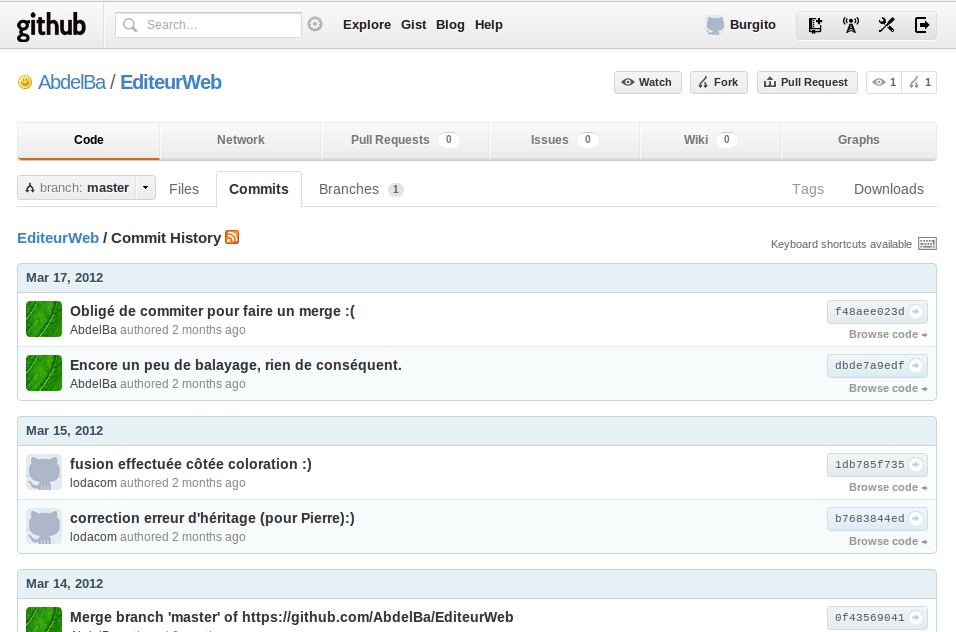
\includegraphics[width=18cm]{images/GitHub.png}
			\caption{Aperçu de notre plateforme GitHub, sur la page des commits}
			\label{commit}
			\end{center}
		\end{figure}	
		\begin{figure}[ht]
			\begin{center}
			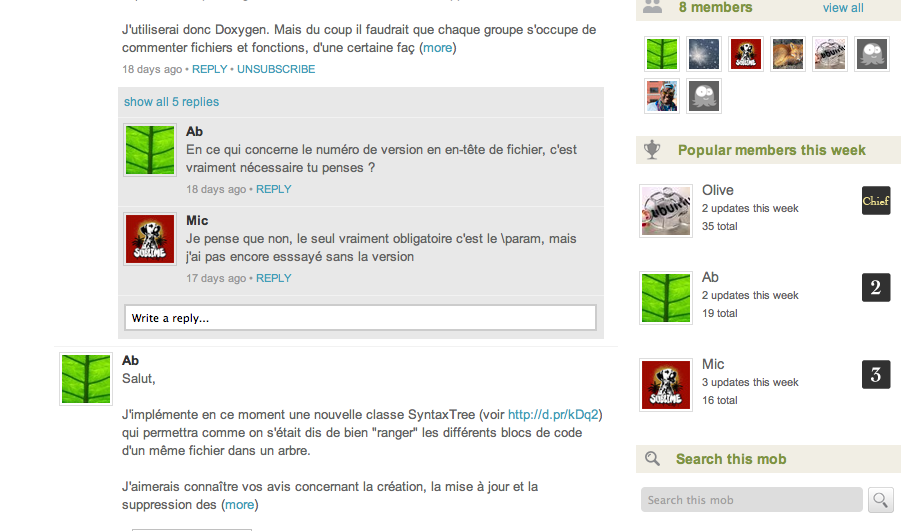
\includegraphics[width=18cm]{images/Micromobs.png}
			\caption{Aperçu de notre plate forme de collaboration Micromobs}
			\label{mmobs}
			\end{center}
		\end{figure}
	\end{section}
	\end{chapter}
%%%%%%%%%%%%%%%%%%%%%%%%%%%%%%%%%%%%%%%%
%%%%%%%%%%%%%%%%%%%%%%%%%%%%%%%%%%%%%%%%
	%% Glossaire
	\renewcommand\glossaryname{Glossaire}
	\renewcommand{\glsnamefont}[1]{\makefirstuc{#1}} % Majuscules.
	\printglossaries
%%%%%%%%%%%%%%%%%%%%%%%%%%%%%%%%%%%%%%%%
%%%%%%%%%%%%%%%%%%%%%%%%%%%%%%%%%%%%%%%%
	%% Sitographie
	\renewcommand\bibname{Sitographie}%% Changement du titre de bibliographie en sitographie.
	\begin{thebibliography}{2}
		\label{sitographie}
		\bibitem{Github}
		Github : www.github.com \\
		Le site spécialisé dans la gestion de dépôts \gls{Git}. Possède une interface très pratique pour gérer les groupes, les projets,
		les fichiers et plus encore.
		~\\
		\bibitem{Wikipedia}
		Wikipédia : www.wikipedia.org \\
		L'encyclopédie en ligne de laquelle j'ai tiré certaines définitions présentes dans le glossaire.
		~\\
		\bibitem{yUML}
		yUML : www.yuml.me \\
		Ce site permet de générer à la volée des diagrammes \gls{UML}, extrêmement utile lorsqu'il s'agit de travail de groupe.
		~\\
		\bibitem{Micromobs}
		Micromobs : www.micromobs.com \\
		Le site de discussion de groupe au principe intéressant : il vaut mieux une interface dédiée aux discussions plutôt
		qu'une boîte e-mail encombrée et mal organisée.
		~\\
		\bibitem{TeamGantt}
		TeamGantt : www.teamgantt.com \\
		Création en ligne de diagrammes de Gantt beaux et lisibles.
		~\\
		\bibitem{Facebook}
		Facebook : www.facebook.com \\
		Le réseau social que l'on ne présente plus, il nous a permis d'échanger des messages moins techniques que sur Micromobs
		et de nous organiser grâce à différents évènements.
		~\\
		\bibitem{Prezi}
		Prezi : www.prezi.com \\
		Un générateur de présentation en ligne nouvelle génération.
		~\\
		\bibitem{Qt Reference Documentation}
		Qt Reference Documentation : www.doc.qt.nokia.com \\
		La documentation Qt, là où nous avons tout appris.	
		~\\
		\bibitem{Stackoverflow}
		Stackoverflow : www.stackoverflow.com \\
		Un forum où sont posés et résolus de nombreux problèmes de programmation. Les personnes qui répondent le font de manière
		très professionnelle ce qui nous a beaucoup aidé.
		~\\
		\bibitem{Le site du zéro}
		Le site du zéro : www.siteduzero.com \\
		Un ensemble bien organisé de cours dans différentes branches de l'informatique et un forum très actif font du site du zéro
		un bon choix pour les débutants.
		~\\
		\bibitem{Developpez.com}
		Developpez.com : www.developpez.com \\
		Ce site est une source inépuisable de données, documentations, questions et réponses concernant la programmation dans tout les langages.
		~\\
		\bibitem{Sourceforge}
		Sourceforge : www.sourceforge.net \\
		Le site de référence en matière de projets open source, c'est ici que nous avons trouvés des exemples de parseurs.
		~\\
		\bibitem{QtFr.org}
		QtFr.org : qtfr.org \\
		Forum de la communauté francophone de Qt, pour les anglophobes.
		\end{thebibliography}
\end{document}
